
\chapter{ارزیابی}

در این مساله هدف بیشینه کردن سود حاصل از پذیرش تقاضاهای زنجیره‌ی کارکرد سرویس می‌باشد که به این ترتیب معیار مقایسه نیز همین پارامتر خواهد بود. این پارامتر در ارزیابی با سایر مقالات مقایسه می‌شود ولی باید در نظر داشت که نیازمندی‌های مدیریتی که در این پژوهش مدنظر است در سایر پژوهش‌ها مدنظر نبوده است.
راه‌حل پیشنهادی بهینه نبوده و به همین علت کارآیی آن در سناریوهایی با حل بهینه مقایسه می‌شود.
سایر پارامترهایی چون تعداد زنجیره‌های پذیرفته شده و ... نیز در این پژوهش ارزیابی می‌گردند.

\section{مقدمه}

همانطورکه پیشتر بیان شد مساله‌ی اصلی راه‌حل چندجمله‌ای ندارد. این مساله با استفاده از چهارچوب \lr{CPLEX} و با زبان جاوا
توسعه یافته است. چهارچوب \lr{CLPEX} توسط شرکت \lr{IBM} توسعه پیدا کرده است و برای حل مسائل خطی استفاده می‌گردد. این
چهارچوب به صورت کلی برای حل مسائل \lr{ILP} از روش \lr{B\&C} استفاده می‌کند. پیاده‌سازی فرمول‌بندی این مساله در این چهارچوب
در پیوست آمده است.

\section{محیط ارزیابی}
به صورت کلی در تمامی ارزیابی‌های این رساله از دو توپولوژی \lr{FatTree} و \lr{USnet} استفاده شده است.
توپولوژی \lr{FatTree} یک توپولوژی سازمان‌یافته است که در ادامه ساختار آن را می‌بینید.


\begin{figure}[!h]
\center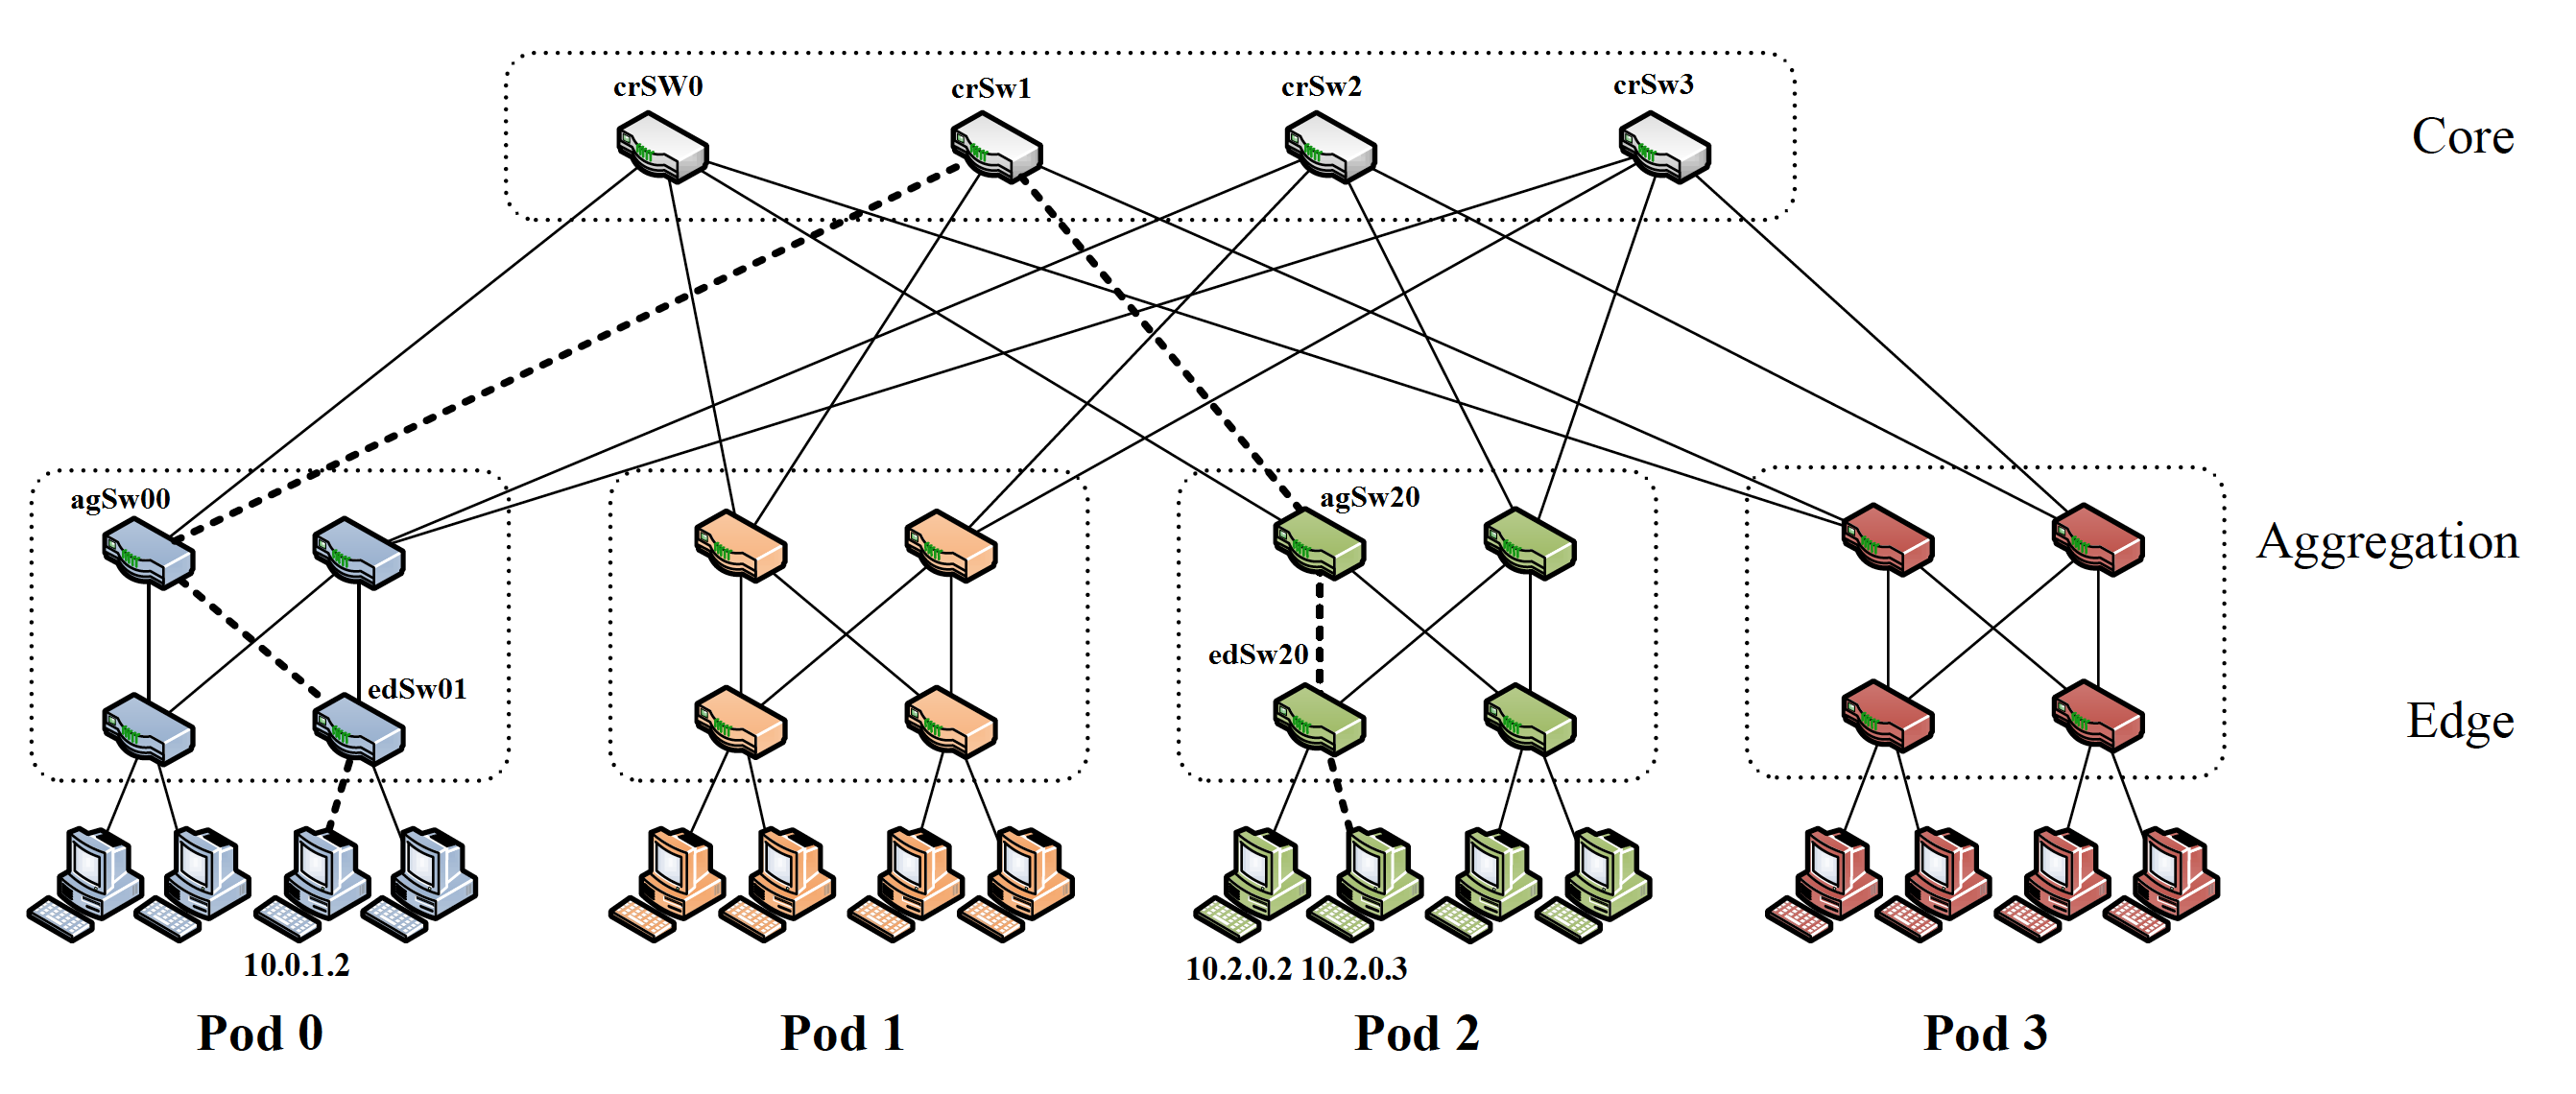
\includegraphics[scale=.25]{images/fattree}
\caption{توپولوژی ساختاریافته \lr{FatTree}}
\label{fig.2}
\end{figure}

توپولوژی \lr{FatTree} با مقدار \(k\) یک توپولوژی ۳ لایه (هسته، تجمعی و لبه) می‌باشد که:
\begin{itemize}
    \item هر غلاف از \((k/2)^2\) سرور و ۲ لایه \(k/2\)تایی سوئیچ \(k\) پورت تشکیل شده است.
    \item هر سوئیچ لبه به \(k/2\) سرور و \(k/2\) سوئیچ تجمعی متصل است.
    \item هر سوئیچ تجمعی به \(k/2\) سوئیچ لبه و \(k/2\) سوئیچ هسته متصل است.
    \item \((k/2)^2\) سوئیچ هسته که هر کدام به \(k\) غلاف متصل هستند.
    \item سوئیچ‌های هسته گره‌های ورودی و خروجی این توپولوژی هستند.
\end{itemize}
در این توپولوژی فرض می‌کنیم مدیریت هر غلاف تنها می‌تواند در همان غلاف یا غلاف‌های همسایه صورت بگیرد.

توپولوژی \lr{USnet} یک تولوپوژی تصادفی می‌باشد که از ۲۴ نود و ۴۳ لینک تشکیل شده است.
در پیاده‌سازی فرض شده است که همه‌ی ۲۴ نود سوئیچ هستند و می‌توانند به عنوان گره‌ی ورودی و خروجی اعمال نقش کنند.
این توپولوژی دیتاسنتری نبوده و سرور‌ها به صورت تصادفی به سوئیچ‌ها متصل می‌شوند که باعث می‌شود
این توپولوژی ماهیت تصادفی داشته باشد.

\begin{figure}[!h]
\center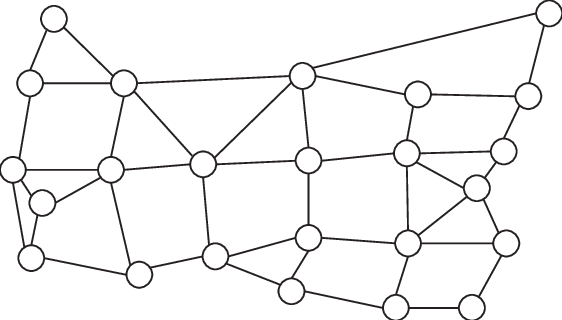
\includegraphics[scale=.5]{images/usnet}
\caption{توپولوژی تصادفی \lr{USnet}}
\label{fig.3}
\end{figure}

\section{معیار‌های ارزیابی}

همانطور که پیشتر بیان شد معیار اصلی ارزیابی سود حاصل از جایگذاری زنجیره‌ها می‌باشد.
پارامترهای زیادی در مساله موثر هستند که در این قسمت به مرور آن‌ها می‌پردازیم.

\subsection{نسبت سود به هزینه}

یکی از ویژگی‌های مهم مساله‌ای طرح شده در نظر گرفتن نیازمندی‌های مدیریتی است. یکی از این نیازمندی‌ها که در تابع هدف هم
وجود دارد نیاز به تهیه گواهی برای هر \lr{VNFM} است.
این گواهی هزینه‌ای در بردارد و نیاز است که از آن به درستی استفاده شود
و تاجایی که امکان دارد \lr{VNFM} با ظرفیت خالی نداشت.

برای اینکه تخمین درستی از این پارامتر داشته باشیم و بتوانیم از آن در ارزیابی‌های پیش رو استفاده کنیم، موارد زیر را تعریف می‌کنیم:
    

\begin{latin}
    \begin{align}
      licenseFee / capacity = \text{amortized license cost per instance}
    \end{align}
    \begin{align}
      chainPrice / chainLength = \text{amortized price per instance}
    \end{align}
    \begin{align}
      \text{amortized price per instance} - \text{amortized license cost per instance} = \text{instance profit} 
    \end{align}
\end{latin}

در نهایت یکی از پارامترهایی که برای ارزیابی راه‌حل پیشنهادی وجود دارد
نسبت سود نمونه به هزینه سرکشن شده گواهی برای هر نمونه می‌باشد.
در زمانی که این نسبت عددی کوچک است استفاده نادرست از گواهی‌ها ضرر زیادی می‌زند و شاید بهتر باشد زنجیره‌های کمتری پذیرفته شوند.
در حالتی که این نسبت عدد بزرگی باشد می‌توان از این هزینه‌ها صرفنظر کرده و تنها منابع مصرفی اجزای مدیریتی مدنظر خواهند بود.
در ادامه از این پارامتر تحت عنوان نسبت سود به هزینه یاد می‌کنیم.

\subsection{سود}

سود، اختلاف میان مجموع قیمت زنجیره‌های پذیرفته شده و هزینه‌هایی است که برای گواهی‌ها پرداخت شده است. سود دقیقا همان تابع هدف مساله است که ارزیابی بر اساس آن صورت می‌گیرد. قیمت زنجیره‌ها پیش از جایگذاری آن‌ها مشخص شده است و فرض می‌کنیم این قیمت با تعداد نمونه‌های داخل زنجیره نسبت مستقیم دارد.

\subsection{تعداد زنجیره‌های پذیرفته شده}

تعداد زنجیره‌هایی است که جایگذاری آن‌ها با موفقیت انجام شده و برای آن‌ها منابع مدیریت نیز تخصیص داده شده است. این معیار در زمانی که پارامتر نسبت سود به هزینه پایین باشد نمود خوبی از عملکرد الگوریتم نمی‌باشد.

\subsection{تعداد \lr{VNFM}های استفاده شده}

تعداد \lr{VNFM}هایی که برای مدیریت زنجیره‌ها تخصیص داده می‌شوند نمایش دهنده‌ی تعداد گواهی‌های استفاده شده است.
این معیار در زمانی که پارامتر نسبت سود به هزینه بالا باشد نمود خوبی از عملکرد الگوریتم نمی‌باشد.

\section{محیط ارزیابی}

برای ارزیابی از زنجیره‌های تصادفی استفاده می‌شود و هر نمونه از ارزیابی میانگین ۱۰ اجرا می‌باشد.
برای تولید زنجیره‌های تصادفی از ابزاری استفاده می‌شود که برای همین پژوهش توسعه یافته است و زنجیره‌های خطی با طول تصادفی تولید می‌کند.
نمونه‌های داخل زنجیره‌ها دارای نوع می‌باشند که به صورت تصافدی از لیست زیر انتخاب می‌شوند:

\begin{latin}
    \begin{verbatim}
types:
  - name: ingress
    cores: 0
    ram: 0
    ingress: true
    manageable: false
  - name: egress
    cores: 0
    ram: 0
    egress: true
    manageable: false
  - name: vFW
    cores: 2
    ram: 2
    manageable: true
  - name: vNAT
    cores: 2
    ram: 4
    manageable: true
  - name: vIDS
    cores: 2
    ram: 2
    manageable: true
  - name: vDPI
    cores: 2
    ram: 4
    manageable: true
    \end{verbatim}
\end{latin}

زنجیره‌های تولید شده دارای گره‌ی آغازی و پایانی می‌باشند
و ترافیک عبوری از آن‌ها ۲۵۰ واحد است.
تنظیمات زیر برای \lr{VNFM}ها در نظر گرفته شده است.

\begin{latin}
    \begin{verbatim}
    ram: 4
    cores: 2
    capacity: 10
    radius: 100
    bandwidth: 1
    licenseFee: 100
    \end{verbatim}
\end{latin}

تنظیمات زیر برای زیرساخت فیزیکی در نظر گرفته شده است:


\begin{latin}
    \begin{verbatim}
    ram: 10 - 48
    cores: 100 - 700
    bandwidth: 40000
    \end{verbatim}
\end{latin}

تمامی ارزیابی‌ها روی سیستمی با مشخصات زیر انجام شده‌اند:

\begin{latin}
    \begin{itemize}
        \item AMD Ryzen Threadripper 1950X 16-Core Processor
        \item 22 GB of RAM
        \item 100 GB of non-SSD Storage
    \end{itemize}
\end{latin}

در نهایت برای بازتولید نتایج تمامی کدها و تنظیمات در \cite{RoadToMSc} موجود است.

\section{نتایج ارزیابی}
ابتدا زمان حل مساله‌ی بهینه و تاثیر نسبت سود به هزینه در مساله را بررسی می‌کنیم.
به این ترتیب می‌توانیم شرایط ارزیابی که در آن عمل می‌کنیم را استدلال کنیم.
در ادامه به گزارش و تحلیل نتایج می‌پردازیم.

\subsection{زمان حل بهینه}
با استفاده از ۱۳۰ زنجیره‌ی تصادفی که طولی بین ۳ تا ۷ دارند
و توپولوژی \lr{FatTree} با مقدار \(k\) برابر ۸ قصد داریم
زمان حل راه حل بهینه و شکاف بهینه\footnote{\lr{Optimality Gap}} آن را ارزیابی کنیم. برای این ارزیابی نسب سود به هزینه برابر ۹ فرض شده است.


\begin{figure}[h]
\center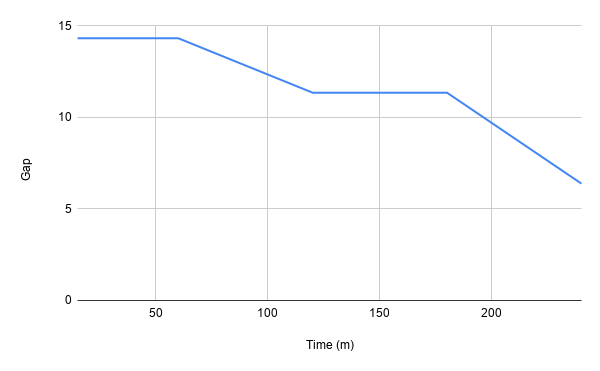
\includegraphics[scale=.5]{images/chart-5}
\caption{شکاف بهینه الگوریتم بهینه بر اساس زمان اجرا (بر حسب دقیقه)}
\label{fig.10}
\end{figure}

شکاف بهینه برای ۱۰۰ زنجیره در ۱۵ دقیقه با شرایط فوق برابر با ۴ درصد می‌باشد بنابراین
در سایر ارزیابی‌ها الگوریتم بهینه را تا ۱۵ دقیقه محدود کرده و تعداد زنجیره‌ها را از ۱۰۰ افزایش نمی‌دهیم.

همانطور که در نمودار \ref{fig.10} مشاهده می‌شود زمان حل مساله‌ی بهینه برای ۱۳۰ زنجیره نسبت به ۱۰۰ زنجیره جهش بزرگی داشته
و بعد از ۴ ساعت ما به شکاف بهینه زیر ۱۰ درصد می‌رسیم.
به این ترتیب استفاده از راه‌حل بهینه ممکن است زمان‌بر باشد و نیاز به پیاده‌سازی یک راه‌حل مکاشفه‌ای می‌باشد.

\subsection{نسبت سود به هزینه}

در ادامه راه‌حل پیشنهادی و راه‌حل \cite{Bari2015} را با نسبت‌های مختلف سود به هزینه مورد آزمون قرار می‌دهیم. 
در این آزمون‌ها از ۱۰۰ زنجیره با طول‌های تصادفی ۳ تا ۷ استفاده می‌کنیم.
توپولوژی مورد استفاده
\lr{FatTree}
با مقدار \(k\)
برابر با ۸
می‌باشد.
در این آزمایش‌ها نسبت سود حاصل از هر الگوریتم به الگوریتم بهینه سنجیده شده و در نمودار آمده است.
در نظر داشته باشید که این نسبت به صورت عددی بین ۰ تا ۱ گزارش شده است.
مساله بهینه با زمان ۱۵ دقیقه محدود شده است.


\begin{figure}[h]
\center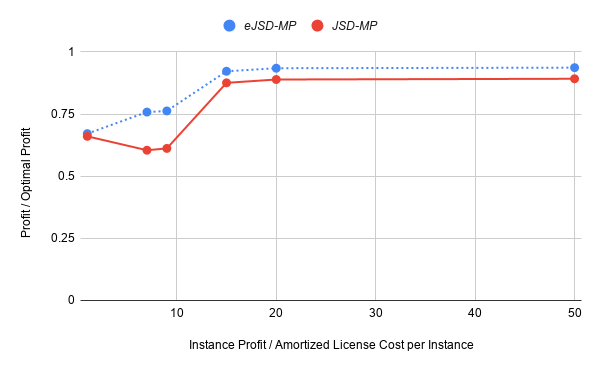
\includegraphics[scale=.5]{images/chart-1}
\caption{کارآیی الگوریتم پیشنهادی و \cite{Bari2015} در نسبت‌های مختلف سود به هزینه}
\label{fig.4}
\end{figure}

همانطور که در نمودار \ref{fig.4} دیده می‌شود الگوریتم پیشنهادی بهتر از الگوریتم \cite{Bari2015} عمل می‌کند.
این امر زمانی که نسبت سود به هزینه بزرگتر است بیشتر دیده می‌شود.
در ادامه برای تمامی ارزیابی‌ها از نسبت سود به هزینه ۹ استفاده می‌کنیم که از نظر فنی عدد معقولی بوده و تاثیر در نظر گرفتن هزینه گواهی را از بین نمی‌برد.

\subsection{زنجیره‌ها در توپولوژی \lr{FatTree}}

در تمامی این ارزیابی‌ها از نسبت سود به هزینه ۹ استفاده کرده و زنجیره‌ها را در توپولوژی \lr{FatTree} جایگذاری می‌کنیم.
در این ارزیابی تعداد زنجیره‌ها را تغییر می‌دهیم اما همواره طول زنجیره‌ها بین ۳ تا ۷ می‌باشد.
همانطور که بیان شد الگوریتم بهینه برای تمامی حالت‌ها تا ۱۵ دقیقه محدود شده است، برای حالت ۱۳۰ برای رسیدن به شکاف بهینه زیر ۱۰ درصد نیاز به ۴ ساعت زمان است.


\begin{figure}[h!]
\center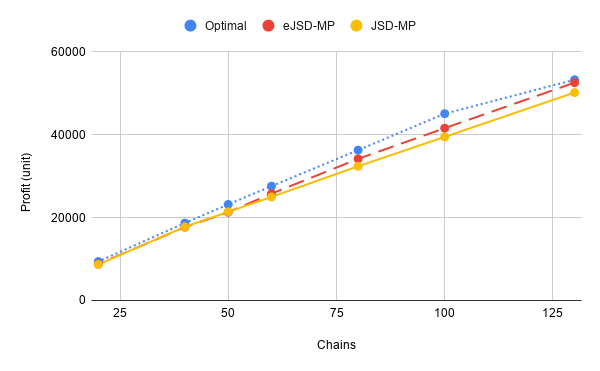
\includegraphics[scale=.5]{images/chart-2}
\caption{سود نهایی الگوریتم‌های بهینه، پیشنهادی و \cite{Bari2015} برای توپولوژی \lr{FatTree}}
\label{fig.7}
\end{figure}

همانطور که در نمودار \ref{fig.7} مشخص است با افزایش تعداد زنجیره‌ها الگوریتم \cite{Bari2015} از الگوریتم پیشنهادی بدتر عمل می‌کند،
به این ترتیب که سود حاصل از پذیرفتن زنجیره‌ها در الگوریتم پیشنهادی بیشتر است.
یکی از موارد مهم در زمانی که ۱۳۰ زنجیره وجود دارد نزدیکی جواب بهینه به جواب الگوریتم پیشنهادی است.
در این حالت به علت پیچیدگی مساله همانطور که صحبت شد تولید جواب با شکاف بهینه مناسب زمان زیادی می‌برد،
بنابراین جوابی که در این حالت استفاده شده است نسبت به سایر نقاط ۲ درصد شکاف بهینه بیشتری دارد.

الگوریتم پیشنهادی به طور میانگین ۵ درصد از الگوریتم \cite{Bari2015}
بهتر عمل کرده و سود خالص بیشتری تولید می‌کند.
دلیل این بهبود در سود نهایی به خاطر مرتب‌سازی زنجیره‌ها بر اساس قیمت آن‌ها می‌باشد.
الگوریتم پیشنهادی پیش از جایگذاری زنجیره‌ها، آن‌ها را بر اساس قیمت‌شان مرتب می‌کند
که این امر به آن اجازه می‌دهد در زمانی که هنوز زیرساخت خالی است زنجیره‌هایی که سود بیشتری دارند را جایگذاری نماید.
در حالی که الگوریتم \cite{Bari2015}
زیرساخت را با زنجیره‌هایی که سود زیادی ندارند پر کرده و امکان جایگذاری زنجیره‌های پر سود را از دست می‌هد.
همانطور که پیشتر نیز بیان شده بود، روند دو الگوریتم با افزایش تعداد زنجیره‌ها سعودی بوده و جواب حاصل هر دو از جواب بهینه فاصله
زیادی نمی‌گیرد.


\begin{figure}[h!]
\center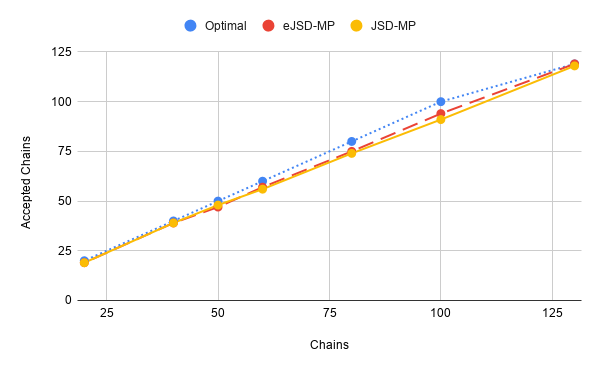
\includegraphics[scale=.5]{images/chart-3}
\caption{تعداد زنجیره‌های پذیرفته شده الگوریتم‌های بهینه، پیشنهادی و \cite{Bari2015} برای توپولوژی \lr{FatTree}}
\label{fig.8}
\end{figure}

\begin{figure}[h!]
\center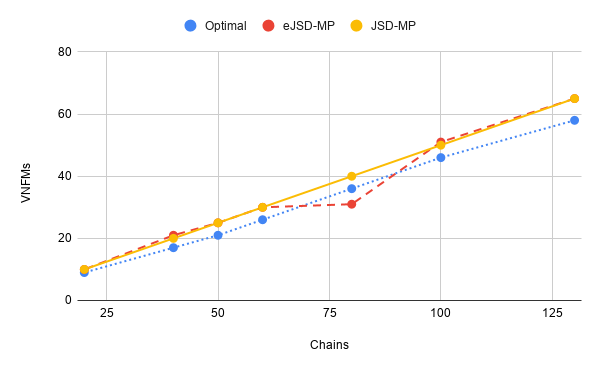
\includegraphics[scale=.5]{images/chart-4}
\caption{تعداد \lr{VNFM}های الگوریتم‌های بهینه، پیشنهادی و \cite{Bari2015} برای توپولوژی \lr{FatTree}}
\label{fig.9}
\end{figure}

نمودارهای \ref{fig.8} و \ref{fig.9}
بیشتر جنبه‌ی اطلاعی دارند و تعداد زنجیره‌های پذیرفته شده و تعداد
\lr{VNFM}های
استفاده شده را نشان می‌دهند.
همانطور که در تعریف مساله نیز گفته شده است، این دو پارامتر در سود نهایی تاثیر دارند
اما سود نهایی به ضرایب آن‌ها نیز وابسته است.

\subsection{زنجیره‌ها در توپولوژی \lr{USnet}}

در تمامی این ارزیابی‌ها از نسبت سود به هزینه ۹ استفاده کرده و
زنجیره‌ها را در توپولوژی \lr{USnet} جایگذاری می‌کنیم.
در این ارزیابی‌ها تعداد زنجیره‌ها را تغییر می‌دهیم اما همواره طول زنجیره‌ها بین ۳ تا ۷ می‌باشد.


\begin{figure}[h!]
\center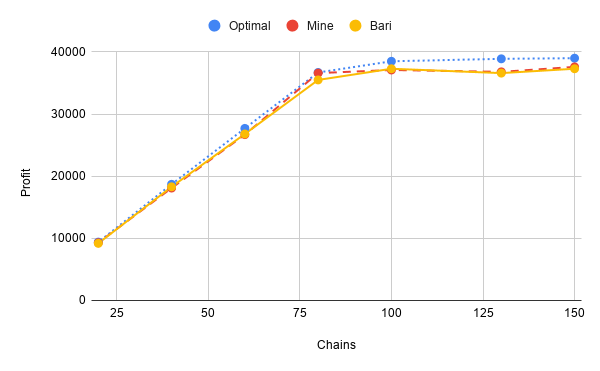
\includegraphics[scale=.5]{images/chart-6}
\caption{سود نهایی الگوریتم‌های بهینه، پیشنهادی و \cite{Bari2015} برای توپولوژی \lr{USnet}}
\label{fig.11}
\end{figure}

از آنجایی که تعداد لینک‌ها و نودهای این توپولوژی کم می‌باشد الگوریتم‌های پیشنهادی و \cite{Bari2015} هر دو مشابه یکدیگر عمل می‌کنند
که این امر در نمودار \ref{fig.11}
نیز قابل رویت است.
اگر بخواهیم این امر را دقیق‌تر بررسی کنیم در این توپولوژی ظرفیت کم بوده و نمی‌توان تعداد زیادی از زنجیره‌های پرسود
را جایگذاری کرد این در حالی است که این توپولوژی محدودیت خاصی برای جایگذاری منابع مدیریتی ندارد
پس می‌توان به سادگی منابع مدیریتی را جایگذاری کرد.
با این تفاسیر مرتب‌سازی اولیه باعث می‌شود که به علت نبود منابع کافی تعداد کمی زنجیره‌ی پر سود جایگذاری شوند.
این در حالی است که الگوریتم \cite{Bari2015}
تعداد زنجیره‌های کوچک بیشتری را جایگذاری می‌کند و منابع مدیریتی را نیز به سادگی به آن‌ها تخصیص می‌دهد.


\begin{figure}[h!]
\center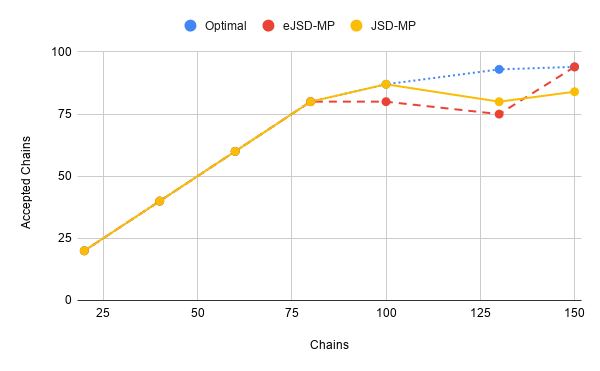
\includegraphics[scale=.5]{images/chart-7}
\caption{تعداد زنجیره‌های پذیرفته شده الگوریتم‌های بهینه، پیشنهادی و \cite{Bari2015} برای توپولوژی \lr{USnet}}
\label{fig.12}
\end{figure}

\begin{figure}[h!]
\center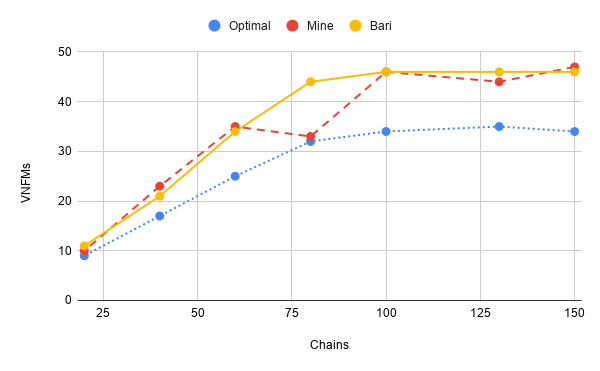
\includegraphics[scale=.5]{images/chart-8}
\caption{تعداد \lr{VNFM}های الگوریتم‌های بهینه، پیشنهادی و \cite{Bari2015} برای توپولوژی \lr{USnet}}
\label{fig.13}
\end{figure}

نمودارهای \ref{fig.13} و \ref{fig.12}
بیشتر جنبه‌ی اطلاعی دارند و تعداد زنجیره‌های پذیرفته شده و تعداد
\lr{VNFM}های
استفاده شده را نشان می‌دهند.
همانطور که در تعریف مساله نیز گفته شده است، این دو پارامتر در سود نهایی تاثیر دارند
اما سود نهایی به ضرایب آن‌ها نیز وابسته است.

\section{ارزیابی زمان اجرا}

همانطور که پیشتر بیان شده بود یکی از بهبودهای الگوریتم پیشنهادی نسبت به
الگوریتم \cite{Bari2015}
زمان اجرای آن می‌باشد.
در این قسمت قصد داریم این موضوع را مورد آزمایش قرار دهیم.
به این منظور از توپولوژی \lr{FatTree} با مقدار \(k\) برابر با ۱۰ استفاده می‌کنیم.
با توجه به ابعاد این توپولوژی امکان حل آن با الگوریتم بهینه بر روی سیستم پیشنهادی وجود دارد ندارد.

در این ارزیابی از ۱۰۰ زنجیره‌ی ورودی استفاده می‌شود. الگوریتم پیشنهادی
در زمان ۵ دقیقه ۱۰۰ زنجیره را جایگذاری کرده و از ۳۳ نمونه
\lr{VNFM}
استفاده می‌کند. در حالی که الگوریتم \cite{Bari2015}
در زمان ۷ دقیقه تنها ۹۹ زنجیره را جایگذاری کرده و از ۵۳ نسخه
\lr{VNFM}
استفاده می‌کند.

همانطور که بیان شد، با توجه به اینکه در ابتدای امر تمامی زیرساخت خالی می‌باشد
می‌توان از یک الگوریتم ساده برای جایگذاری استفاده کرد و به این ترتیب
بدون تاثیر در جواب نهایی زمان حل مساله را کاهش داد.

در این حالت ۲۰ زنجیره‌ی ابتدایی به صورت \lr{first-fit}
جایگذاری شدند.


\section{جمع‌بندی}
در این فصل راه‌حل پیشنهادی را ارزیابی کرده و نشان دادیم
که این راه‌حل به طور میانگین برای توپولوژی‌های \lr{FatTree} و \lr{USnet}
۹۰ درصد جواب بهینه را ارائه می‌دهد.
در ادامه نشان داده شد این الگوریتم از الگوریتم \cite{Bari2015}
در توپولوژی \lr{FatTree}
به صورت میانگین ۵ درصد بهتر عمل می‌کند.
و در توپولوژی \lr{USnet}
به طور میانگین ۱ درصد بهبود عملکرد دارد.

در ادامه در ارزیابی‌ها نشان داده شد که این الگوریتم پیشنهادی برای نگاشت منابع مدیریتی
به صورت میانگین ۷۰ درصد الگوریتم بهینه عملکرد دارد
که برای نسبت سود به هزینه‌ای که در عمل وجود دارد عددی مناسب است.